\documentclass[12pt, a4paper, oneside]{article}
%die Pakete werden hier durch den Include-Befehl separat eingelesen
\usepackage[utf8]{inputenc}
\usepackage{amsmath} % Mathematik-Pakete
\usepackage{amsfonts}
%\usepackage{mathptmx} %times new roman
%\usepackage[T1]{fontenc} %vollen Zeichensatz ]
\usepackage{amssymb}
\usepackage[ngerman]{babel}
\usepackage{graphicx}
\usepackage{microtype} %besserer Randausgleich
\usepackage{footnote}
\usepackage{blindtext}
\usepackage{etoolbox}
%\usepackage{makeidx}
%\usepackage{dsfont}
\usepackage{lettrine}%\usepackage{geometry}
%\usepackage{xcolor} % Für verschiedene Farben
\newcommand{\ricardo}[1]{\colorbox{ForestGreen}{\color{white}   \textsf{\textbf{Ricardo}}} \textcolor{ForestGreen}{#1}}
\usepackage[pdfborderstyle={/S/U/W 1}]{hyperref} % Für interaktive Refernzierung im PDF
\usepackage{csquotes}
\usepackage{acro}
\usepackage{hyperref} % Für interaktive Refernzierung im PDF
\usepackage[onehalfspacing]{setspace}%Zeilenabstand 1.5
% \usepackage{picins} % Das Umfließen einer Grafik im Text kann mit dem Paket PicIns erreicht werden.
%\usepackage{fontspec} 

%\usepackage[utf8]{inputenc}
\usepackage[ngerman]{babel}
\usepackage[top=2.5cm, bottom=2.5cm, left=2cm, right=3.5cm]{geometry}
\usepackage{bibgerm}
\usepackage{tabularx}
\usepackage{adjustbox}
\usepackage{cite}
\usepackage{blindtext}
\usepackage{epsfig}
\usepackage{longtable}
%\usepackage{showframe}
\usepackage{dcolumn}%benötigt für stargaze
\usepackage{here}%lädt das Paket zum Erzwinge n der Grafikposition
\usepackage{floatflt}%Bilder im Fließtext
%\usepackage{fontspec}
%\usepackage{fontenc}
\usepackage{dsfont}
%\setsansfont[Ligatures=TeX]{Arial}
%\renewcommand{\familydefault}{\sfdefault}
%\usepackage{times}
\usepackage{graphicx}
\usepackage{epstopdf}

\usepackage{xcolor}
\usepackage{listings}

\usepackage{lipsum}


\usepackage[T1]{fontenc}
\usepackage{lmodern}



\lstset{language=R}
\lstset{basicstyle=\ttfamily,
basicstyle=\small}
\lstset{literate=%
  {Ö}{{\"O}}1
  {Ä}{{\"A}}1
  {Ü}{{\"U}}1
  {ß}{{\ss}}1
  {ü}{{\"u}}1
  {ä}{{\"a}}1
  {ö}{{\"o}}1
}

\title{\textbf{Titel der Arbeit}}
\author{Max Mustermann}

\setlength{\parindent}{0cm} %keine Einrückung
\linespread{1.5} 

\acsetup{first-style=short}
\newpage
\newpage
%Hier fängt die Deklarierung von Akronymen
%in alphabetischer Reihenfolge an
%auf Akronym im Text verweisen mittels \ac{ }
\DeclareAcronym{AIC}{
	short = AIC ,
	long  = \hspace*{22mm}Akaike-Informationskriterium ,
	tag = abbrev
}

\DeclareAcronym{BLES}{
	short = BLES ,
	long  = \hspace*{19mm}Bester Linearer Erwartungstreuer Schätzer ,
	tag = abbrev
}

\DeclareAcronym{c.p.}{
	short = c.p. ,
	long  = \hspace*{22mm}ceteris paribus ,
	tag = abbrev
}


\DeclareAcronym{u.i.v.}{
	short = u.i.v. ,
	long  = \hspace*{22mm}unabhängig und identisch verteilt ,
	tag = abbrev
}

\DeclareAcronym{KQS}{
	short = KQS ,
	long  = \hspace*{20mm}Kleinste-Quadrate-Schätzung ,
	tag = abbrev
}


\DeclareAcronym{VA}{
	short = VA ,
	long  = \hspace*{23mm}Varianzanalyse ,
	tag = abbrev
}


\newpage
\newpage
%in alphabetischer Reihenfolge

\newcounter{SeitenzahlSpeicher}
\begin{document}

 \thispagestyle{empty}
\begin{titlepage}
	 \thispagestyle{empty}
	% thispagestyle{empty} unterdrückt Seitenzahlen auf der gewünschten Seite
	\newfont{\smc}{cmcsc10 at 12pt}
%	\maketitle
	%Aufpassen mit fi: Fehlercode U+FB01
	%%%%%%%%%%%%%%%%%%%%%%%%%%%%%%%%%%%%%%%%%%
%Titel, Autor, Seminar, Semester, Dozent %
%%%%%%%%%%%%%%%%%%%%%%%%%%%%%%%%%%%%%%%%%%
\begin{center}
	 \thispagestyle{empty}
\begin{figure}[t]
	\centering
	
\includegraphics[width=0.6\textwidth]{assets/HTW_Logo.jpg}
	%\includegraphics[width=0.8\textwidth]{UniGoettingen.pdf}
	
\end{figure}

$~~$\\
\textbf{\huge Entwicklung eines Self-Service zur Bewertung digitaler Anwendung auf Verschreibungsfähigkeit }\paragraph{}$~~$\\
%\textbf{\huge Entwicklung eines Self-Service zur Feststellung des DiGA Status einer digitalen Anwendung}\paragraph{}$~~$\\
\paragraph{}$~~$\\
\paragraph{}$~~$\\
\textbf{Forschungsprojekt Teil B}\\ \textbf{an der Hochschule für Technik und Wirtschaft Berlin}
\paragraph{}$~~$\\
\paragraph{}$~~$\\
\paragraph{}$~~$\\
\text{vorgelegt am: \today}\\
\text{von: Miriam Lischke}\\
%\text{aus: Berlin}\\
\text{1. Gutachter: Prof. Dr. Peter Hufnagl}\\
\text{2. Gutachter: M Sc. Thorsten Knape}\\
\paragraph{}$~~$\\
%\text{Hochschule für Technik und Wirtschaft}\\
%\text{Professur für empirische Außenwirtschaft}\\
\end{center}	
\end{titlepage}



\begin{spacing}{1}
\pagenumbering{Roman}
\setcounter{page}{2}
\tableofcontents
\end{spacing}
\newpage
\begin{spacing}{1}
\section*{Abbildungsverzeichnis} 
\addcontentsline{toc}{section}{Abbildungsverzeichnis}
\renewcommand{\listfigurename}{}
\listoffigures
\end{spacing}
\newpage
\section*{Tabellenverzeichnis} 
\addcontentsline{toc}{section}{Tabellenverzeichnis} 
\renewcommand{\listtablename}{}
\listoftables % Tabellenverzeichnis
\footnote{Alle Tabellen wurden eigenständig erstellt, siehe \emph{R}-Code} 
\newpage
\section*{Symbolverzeichnis} 
\addcontentsline{toc}{section}{Symbolverzeichnis} 
%Sortieren nach Auftreten im Text
\begin{table}[h] \begin{center} \begin{tabular}{|lll|} \hline 
& \textbf{Symbol} & \textbf{Bedeutung} \\ \hline \hline
& $H_0 \colon$ &Nullhypothese\\ 
& $H_1 \colon$ &Alternativhypothese\\
& $\mathbf{I}_n\colon$ &Einheitsmatrix der Dimension $n$\\
& $k$ &Anzahl der unabhängigen Variablen\\
& $L(\cdot)$ &Plausibilitätsfunktion bzw. Likelihood-Funktion\\ 
& $\ell(\cdot)$ & logarithmische Plausibilitätsfunktion bzw. log-Likelihood-Funktion\\ 
& $n\colon$& Stichprobenumfang\\
& $p$ &Anzahl der Regressionsparameter\\
& $R^2\colon$ & Bestimmtheitsmaß\\ 
& $\overline{R}^2\colon$ & adjustiertes Bestimmtheitsmaß\\ 
& $\mathbf{X}\colon$& Versuchsplanmatrix \\ 
& $\beta_1,\beta_2, \ldots, \beta_k\colon$& unbekannte Regressionsparameter\\ 
& $ G_\Phi(\vartheta)$& Gütefunktion\\ 
& $\hat{\boldsymbol \beta}\colon$& KQ-Schätzvektor \\ \hline
\end{tabular} \end{center} \end{table}
\newpage
\section*{Abkürzungsverzeichnis} 
\addcontentsline{toc}{section}{Abkürzungsverzeichnis}
%\printacronyms[include-classes=abbrev,name=Abkürzungen]
\newpage
\clearpage
\setcounter{SeitenzahlSpeicher}{\value{page}}
\pagenumbering{arabic}
\newpage
\pagenumbering{arabic}

\section{Einführung}
\subsection{Situationsbeschreibung}
\emph{Im Zuge der zunehmenden Digitalisierung} des Gesundheitswesens, ergeben sich für IT spezialisierte bzw. Unternehmen im Allgemeinen vermehrt Perspektiven in der Gesundheitsbranche fußzufassen. 
Aus diesen neuen Möglichkeiten der Branche entstehen eine Vielzahl an Kooperationen zwischen Experten aus verschiedensten Bereiche, wie etwa: Forschung, Wissenschaft, Public Health und Technologie etc. Dabei entstehen innovative Produkte, die dazu beitragen, das Gesundheitswesen voranzubringen. ``Mit dem Inkrafttreten des Digitale-Versorgung-Gesetzes (DVG) am 19. Dezember 2019 wurde die „App auf Rezept“ für Patientinnen und Patienten in die Gesundheitsversorgung eingeführt. 
Damit haben ca. 73 Millionen Versicherte in der gesetzlichen Krankenversicherung (GKV) einen Anspruch auf eine Versorgung mit digitalen Gesundheitsanwendungen (DiGA), die von Ärzten und Psychotherapeuten verordnet werden können und durch die Krankenkasse erstattet werden.''~\cite{leitfadenfasttrack}  
Dieser neue gesetzliche Rahmen schafft eine enorme Geschäftsnische für Unternehmen. 

Jedoch um für ein Produkt den offiziellen Status einer DiGA\footnote{Digitale Gesundheitsanwendung} zu erhalten muss mittels eines aufwendigen Prüfungsverfahren durch das Bundesinstitut für Arzneimittel und Medizinprodukte (BfArM), nach §139e SGB V ermittelt werden ob alle Voraussetzungen erfüllt sind. Erst nach erfolgreicher Prüfung erfolgt die Aufnahme in ein Verzeichnis für erstattungsfähige digitale Gesundheitsanwendungen (\textit{DiGA-Verzeichnis}~\cite{digaverzeichnis}) des BfArM\footnote{Bundesinstitut für Arzneimittel und Medizinprodukte\label{ftn:bfarm}}.

\subsection{Motivation und Forschungsfragen}
Das Verfahren nachdem das BfArM die potenzielle digitale Gesundheitsanwendung prüft nennt sich Fast-Track-Verfahren und wird durch einen Antrag zur Aufnahme in das DiGA-Verzeichnis angestoßen. Obwohl das Verfahren ``als zügiger ``Fast-Track'' (=schneller Weg) konzipiert''~\cite{digahersteller} ist, beträgt die Bearbeitungszeit drei Monate nach Eingang des vollständigen Antrags.

Zur Orientierung stellt das BfArM, den Antragssteller einen Umfangreichen Leitfaden gemäß § 139e Absatz 8 Satz 1 SGB V zur Verfügung. Dieser wendet sich in erster Linie an die Hersteller, denn die Anforderungen sind sehr hoch.

Der Leitfaden soll das Antragsverfahren in seinen Schritten übersichtlich darstellen und schafft Transparenz über die konkret zu erfüllenden Anforderungen im Verfahren und stellt sicher, dass alle Anträge nach gleichen Maßstäben bearbeitet werden.

Da der Leitfaden eher eine zusammenfassende Darstellung der
Regelungen, die an verschiedenen Stellen im SGB V\footnote{Sozialgesetzbuch, Fünftes Buch - Gesetzliche Krankenversicherung\label{ftn:sgb}}, in der DiGAV\footnote{Digitale-Gesundheitsanwendung-Verordnung\label{ftn:digav}} als auch in den Anlagen zur DiGAV zu finden sind, leistet und somit nur darlegt wie es die normativen Vorgaben aus DVG\footnote{Digitale-Versorgung-Gesetz\label{ftn:dvg}} und DiGAV regelmäßig auslegen.
Können vor allem junge Unternehmen wie Startups schnell den Überblick verlieren ob sie bereits die Voraussetzungen zur Antragsstellung erfüllen oder welche Schritte vorher noch eingeleitet werden müssen. Dies fordert viel Vorbereitung, Geld und Zeit. Da wäre es vom großen Vorteil mittels eines Vorabchecks zu prüfen ob bereits alle Anforderungen für einen erfolgreichen Ausgang der Antragsstellungen erfüllt sind oder in Form einer Roadmap aufweist welche Schritte dazu noch erforderlich sind. Daraus ergeben sich konkret die folgenden Forschungsfragen:
%Andererseits können all diese Anforderungen und zusammenfassenden Darstellungen der Reglungen, die unter anderem an verschiedenen Stellen im SGB V, in der DIGAV und in den Anlagen zur DIGAV zufinden sind vor allem junge Unternehmen wie Startups übervordern. 

%Zur Orientierung stellt das BfArM, den Antragssteller einen Umfangreichen Leitfaden gemäß § 139e Absatz 8 Satz 1 SGB V zur Verfügung, denn die Anforderungen an die Hersteller sind sehr hoch.
\begin{enumerate}
         \item Wie lässt sich aus Sicht des Herstellers, der Prozess zur Feststellung ob ein Potential, der eigenen digitalen Anwendung vorliegt als erstattungsfähigen DiGA eingestuft zu werden, vereinfachen?
         %Lasst sich mittels eines entwickelten digitalen Self-Service (sog. "Fast-Track-Checker"), die Vorbereitung zur Antragsstellung auf Aufnahme einer DIGA in das Verzeichnis, die durch das Fast-Track-Verfahren geprüft wird, für Antragssteller bzw. Hersteller vereinfachen?
         \item Wie kann man ein Self-Service verwirklichen, der zur Vereinfachung des Fast-Track-Verfahren bei trägt?
         %der durch den Self-Service entstehenden DiGA-Canvas, zu einer druckfähigen PDF generiert werden, sodass er für Hersteller zur Übersicht der aktuellen Situation und Hilfestellung für die folgenden Schritte dient?
\end{enumerate}

\subsection{Vorgehensweise}
Ziel dieser Forschungsarbeit ist es ein digitalen Self-Service zu entwickeln, der bei der Vorbereitung zum Antrag auf Aufnahme in das DiGA-Verzeichnis unterstützt und mithilfe eines DiGA-Canvas, die Anforderungen und Voraussetzungen kompakt zusammenfässt. Dabei wird ausgiebig erforscht, wie sich die Prüfung durch das Fast-Track-Verfahren zusammensetzt und welche Anforderungen sich dabei an die Hersteller und die Anwendung richten. Des Weiteren wird erforscht welche relevanten Informationen auf dem DiGA-Canvas zur Übersicht zusammengefasst werden sollten und mithilfe welcher Technologie, eine druckfähige PDF generiert werden kann.

\section{App auf Rezept}
Wie bereits erwähnt würde am 19.Dezember 2019 mit der Inkraftsetzung des Digitale-Versorgungs-Gesetzes (DVG), die ``App auf Rezept'' für Patientinnen und Patienten in die Gesundheitsverordnung eingeführt. Digitale Gesundheitsanwendungen (DiGA) können somit von Ärzten und Psychotherapeuten verordnet und durch die Krankenkasse erstattet werden. Dies eröffnet vielfältige Möglichkeiten, um bei der Erkennung und Behandlung von Krankheiten sowie auf dem Weg zu einer selbstbestimmten gesundheitsförderlichen Lebensführung zu unterstützen.

``Das BfArM hat diesen bedeutenden Baustein der Digitalisierungsstrategie der Bundesregierung und des Bundesgesundheitsministeriums von Anfang an mitgestaltet und unterstützt Hersteller und Anwender digitaler Medizinprodukte wie z.B. Medical Apps seit Jahren intensiv u.a. bei Fragen zur Einstufung einer App als Medizinprodukt oder zur Cybersicherheit von Medizinprodukten.'' /cite(https://diga.bfarm.de/de)

``Das Bundesinstitut für Arzneimittel und Medizinprodukte (BfArM) ist eine selbstständige Bundesoberbehörde im Geschäftsbereich des Bundesministeriums für Gesundheit (BMG). [... Es hat in diesem Kontext] die Aufgabe, Anträge zur Aufnahme von DiGA in das Verzeichnis wissenschaftlich zu bewerten. Es stellt außerdem das Verzeichnis für digitale Medizinprodukte bereit, die nach erfolgreicher Prüfung als erstattungsfähige digitale Gesundheitsanwendungen (DiGA) gelistet werden'' /cite(https://diga.bfarm.de/de)

Über sogenannte ``Bekanntmachungen'' im Bundesanzeiger, die erstmals am \textit{06.1.2020}~\cite{https://diga.bfarm.de/assets/documents/201006_BfArM_Bekanntmachung-DiGA-1.pdf} und zuletzt am \textit{29.12.2020}~\cite{https://diga.bfarm.de/assets/documents/201229_BfArM_Bekanntmachung-DiGA-2.pdf} erschienen sind, werden Informationen wie die Errichtung des Verzeichnisses für digitale Gesundheitsanwendungen (DiGA), die Bildung neuer Gruppen oder die Veränderung bestehender Gruppen im DiGA-Verzeichnis, die Aufnahme neuer DiGA im DiGA-Verzeichnis, die Streichung von DiGA aus dem DiGA-Verzeichnis veröffentlicht. Diese Veröffentlichung folgt vierteljährlich.

Für ärztliche oder psychotherapeutische Leistungserbringer eröffnet das Verzeichnis vielfältige Möglichkeiten, sich einen Überblick über verfügbare DiGA zu verschaffen, die möglicherweise für ihre Patienten infrage kommen könnten. Die im Verzeichnis aufgeführten Informationen sollen das gemeinsame aussuchen mit dem Patienten, unterstützen. Sodass die zur aktuellen Situation am besten geeignete DiGA verordnet werden kann.

\subsection{Wie kann eine DiGA verordnet werden?}

\begin{figure}[H]
	\centering
	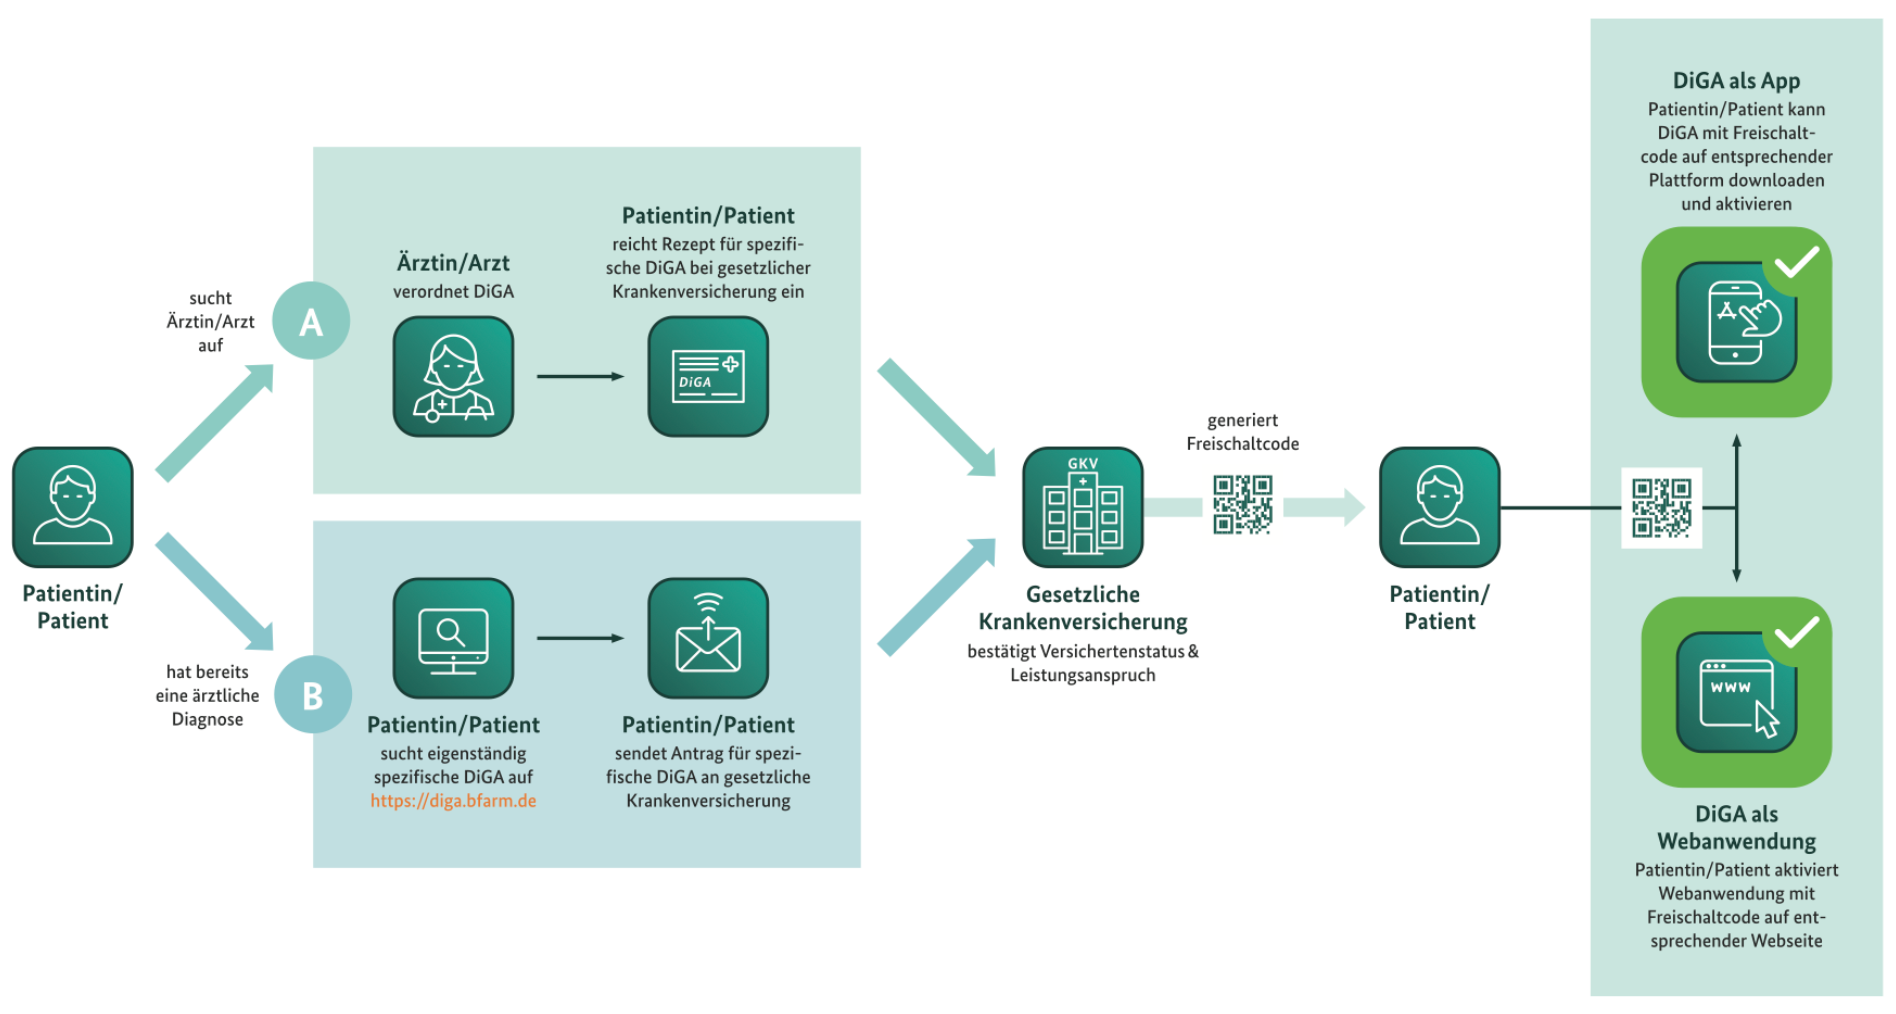
\includegraphics[width=450px, keepaspectratio]{assets/verordnungs_prozess.png}
	\caption{Graphauswertung - Komponentendiagramm,\\Quelle: Eigene Darstellung, Tool: \cite{visual_paradigm}}
\end{figure}
%Kern des Verfahrens sind die Prüfung der Herstellerangaben zu den geforderten Produkteigenschaften – vom Datenschutz bis zur Benutzerfreundlichkeit – sowie die Prüfung eines durch den Hersteller beizubringenden Nachweises für die mit der DiGA realisierbaren positiven Versorgungseffekte. Das sind Effekte, durch die sich der gesundheitliche Zustand eines Patienten oder die Möglichkeiten zum Umgang mit seiner Erkrankung durch die Benutzung der DiGA verbessern.
%
\begin{small}
\begin{quote}
"`Lorem ipsum dolor sit amet, consectetur adipisici elit, sed eiusmod tempor incidunt ut labore et dolore magna aliqua. Ut enim ad minim veniam, quis nostrud exercitation ullamco laboris nisi ut aliquid ex ea commodi consequat. Quis aute iure reprehenderit in voluptate velit esse cillum dolore eu fugiat nulla pariatur. Excepteur sint obcaecat cupiditat non proident, sunt in culpa qui officia deserunt mollit anim id est laborum."' (übersetzt durch Autor)\footnote{Bei Überzetzungen sollte genannt werden, ob es sich um eine in der Literatur rezipierte Übersetzung handelt, oder ob es sich um ein Eigenübersetzung des Autors handelt}
\end{quote}
\end{small}
%
Lorem ipsum dolor sit amet, consectetur adipisici elit, sed eiusmod tempor incidunt ut labore et dolore magna aliqua. Ut enim ad minim veniam, quis nostrud exercitation ullamco laboris nisi ut aliquid ex ea commodi consequat. Quis aute iure reprehenderit in voluptate velit esse cillum dolore eu fugiat nulla pariatur. Excepteur sint obcaecat cupiditat non proident, sunt in culpa qui officia deserunt mollit anim id est laborum.\\

\subsection{Wie funktioniert das Fast-Track- Verfahren?}

\begin{figure}[H]
	\centering
	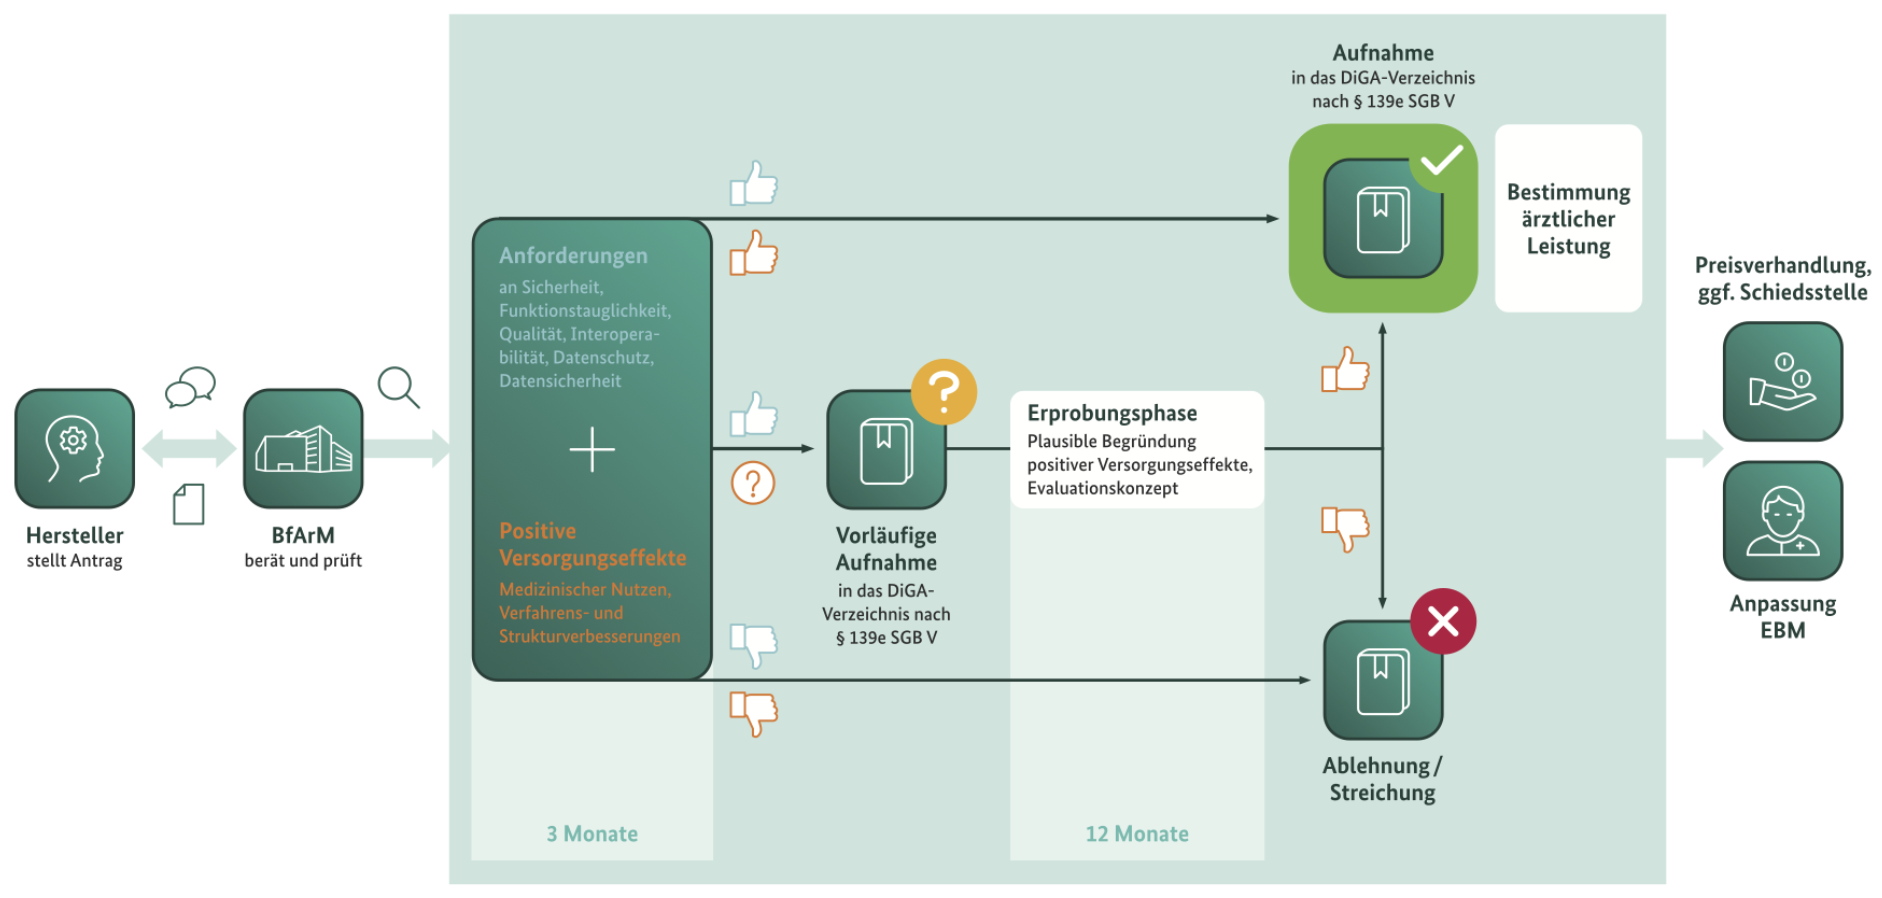
\includegraphics[width=450px, keepaspectratio]{assets/fastTrack_prozess.png}
	\caption{Graphauswertung - Komponentendiagramm,\\Quelle: Eigene Darstellung, Tool: \cite{visual_paradigm}}
\end{figure}
Lorem ipsum dolor sit amet, consectetur adipisici elit, sed eiusmod tempor incidunt ut labore et dolore magna aliqua. Ut enim ad minim veniam, quis nostrud exercitation ullamco laboris nisi ut aliquid ex ea commodi consequat. Quis aute iure reprehenderit in voluptate velit esse cillum dolore eu fugiat nulla pariatur. Excepteur sint obcaecat cupiditat non proident, sunt in culpa qui officia deserunt mollit anim id est laborum.

\subsection{Probleme bei der Analyse des Arbitrageverhaltens}
Lorem ipsum dolor sit amet, consectetur adipisici elit, sed eiusmod tempor incidunt ut labore et dolore magna aliqua. Ut enim ad minim veniam, quis nostrud exercitation ullamco laboris nisi ut aliquid ex ea commodi consequat. Quis aute iure reprehenderit in voluptate velit esse cillum dolore eu fugiat nulla pariatur. Excepteur sint obcaecat cupiditat non proident, sunt in culpa qui officia deserunt mollit anim id est laborum.\\
%
\begin{enumerate}
 \item Lorem ipsum
\item dolor sit amet, consectetur adipisici elit
\item sed eiusmod tempor incidunt ut labore et dolore magna aliqua
\end{enumerate}
%
Lorem ipsum dolor sit amet, consectetur adipisici elit, sed eiusmod tempor incidunt ut labore et dolore magna aliqua. Ut enim ad minim veniam, quis nostrud exercitation ullamco laboris nisi ut aliquid ex ea commodi consequat. Quis aute iure reprehenderit in voluptate velit esse cillum dolore eu fugiat nulla pariatur. Excepteur sint obcaecat cupiditat non proident, sunt in culpa qui officia deserunt mollit anim id est laborum.\footnote{Lorem ipsum dolor sit amet, consectetur adipisici elit, sed eiusmod tempor incidunt ut labore et dolore magna aliqua.} Lorem ipsum dolor sit amet, consectetur adipisici elit, sed eiusmod tempor incidunt ut labore et dolore magna aliqua. Ut enim ad minim veniam, quis nostrud exercitation ullamco laboris nisi ut aliquid ex ea commodi consequat. Quis aute iure reprehenderit in voluptate velit esse cillum dolore eu fugiat nulla pariatur. Excepteur sint obcaecat cupiditat non proident, sunt in culpa qui officia deserunt mollit anim id est laborum.

\section{Klassifikation}
Lorem ipsum dolor sit amet, consectetur adipisici elit, sed eiusmod tempor incidunt ut labore et dolore magna aliqua. Ut enim ad minim veniam, quis nostrud exercitation ullamco laboris nisi ut aliquid ex ea commodi consequat. Quis aute iure reprehenderit in voluptate velit esse cillum dolore eu fugiat nulla pariatur. Excepteur sint obcaecat cupiditat non proident, sunt in culpa qui officia deserunt mollit anim id est laborum.a
\subsection{Anwendungen von Arbitragestrategien}
Lorem ipsum dolor sit amet, consectetur adipisici elit, sed eiusmod tempor incidunt ut labore et dolore magna aliqua. Ut enim ad minim veniam, quis nostrud exercitation ullamco laboris nisi ut aliquid ex ea commodi consequat. Quis aute iure reprehenderit in voluptate velit esse cillum dolore eu fugiat nulla pariatur. Excepteur sint obcaecat cupiditat non proident, sunt in culpa qui officia deserunt mollit anim id est laborum. (siehe \autoref{fig:Abbildung 2}).
%

%
Lorem ipsum dolor sit amet, consectetur adipisici elit, sed eiusmod tempor incidunt ut labore et dolore magna aliqua. Ut enim ad minim veniam, quis nostrud exercitation ullamco laboris nisi ut aliquid ex ea commodi consequat. Quis aute iure reprehenderit in voluptate velit esse cillum dolore eu fugiat nulla pariatur. Excepteur sint obcaecat cupiditat non proident, sunt in culpa qui officia deserunt mollit anim id est laborum.

\subsection{Auswirkungen von Arbitragestrategien}
ALorem ipsum dolor sit amet, consectetur adipisici elit, sed eiusmod tempor incidunt ut labore et dolore magna aliqua. Ut enim ad minim veniam, quis nostrud exercitation ullamco laboris nisi ut aliquid ex ea commodi consequat. Quis aute iure reprehenderit in voluptate velit esse cillum dolore eu fugiat nulla pariatur. Excepteur sint obcaecat cupiditat non proident, sunt in culpa qui officia deserunt mollit anim id est laborum. $300$--$500$ km.\\
\\
Lorem ipsum dolor sit amet, consectetur adipisici elit, sed eiusmod tempor incidunt ut labore et dolore magna aliqua. Ut enim ad minim veniam, quis nostrud exercitation ullamco laboris nisi ut aliquid ex ea commodi consequat. Quis aute iure reprehenderit in voluptate velit esse cillum dolore eu fugiat nulla pariatur. Excepteur sint obcaecat cupiditat non proident, sunt in culpa qui officia deserunt mollit anim id est laborum.

\subsection{Ziele von Arbitragestrategien}
Lorem ipsum dolor sit amet, consectetur adipisici elit, sed eiusmod tempor incidunt ut labore et dolore magna aliqua. Ut enim ad minim veniam, quis nostrud exercitation ullamco laboris nisi ut aliquid ex ea commodi consequat. Quis aute iure reprehenderit in voluptate velit esse cillum dolore eu fugiat nulla pariatur. Excepteur sint obcaecat cupiditat non proident, sunt in culpa qui officia deserunt mollit anim id est laborum.\\

\subsection{Aufbau von Arbitragestrategien}
Lorem ipsum dolor sit amet, consectetur adipisici elit, sed \underline{eiusmod} tempor incidunt ut labore et dolore magna aliqua. Ut enim ad minim veniam, quis nostrud exercitation ullamco laboris nisi ut aliquid ex ea commodi consequat. Quis aute iure reprehenderit in voluptate velit esse cillum dolore eu fugiat nulla pariatur. Excepteur sint obcaecat cupiditat non proident, sunt in culpa qui officia deserunt mollit anim id est laborum:``Lorem ipsum''.

\renewcommand{\labelenumi}{\roman{enumi})}
\begin{enumerate}
\item Lorem ipsum
\item dolor sit amet, consectetur adipisici elit
\item sed eiusmod tempor incidunt ut labore et dolore magna aliqua
\item ullamco laboris nisi ut aliquid
\item ex ea commodi
\item consequat
\end{enumerate}

\setcounter {footnote} {0}
\section{Datenaufbereitung}
Lorem ipsum dolor sit amet, consectetur adipisici elit, sed eiusmod tempor incidunt ut labore et dolore magna aliqua. Ut enim ad minim veniam, quis nostrud exercitation ullamco laboris nisi ut aliquid ex ea commodi consequat. Quis aute iure reprehenderit in voluptate velit esse cillum dolore eu fugiat nulla pariatur. Excepteur sint obcaecat cupiditat non proident, sunt in culpa qui officia deserunt mollit anim id est laborum
%
\begin{quote}
"`Lorem ipsum dolor sit amet, consectetur adipisici elit, sed eiusmod tempor incidunt ut labore et dolore magna aliqua. Ut enim ad minim veniam, quis nostrud exercitation ullamco laboris nisi ut aliquid ex ea commodi consequat. Quis aute iure reprehenderit in voluptate \& velit esse cillum dolore eu fugiat nulla pariatur. Excepteur sint obcaecat cupiditat non proident, sunt in culpa qui officia deserunt mollit anim id est laborum?"' (übersetzt durch Autor)
\end{quote}
%
Lorem ipsum dolor sit amet, consectetur adipisici elit (\texttt{Variable1}, \texttt{Variable2}, \texttt{Variable3}) sed eiusmod tempor incidunt ut labore et dolore magna aliqua. Ut enim ad minim veniam, quis nostrud exercitation ullamco laboris nisi ut aliquid ex ea commodi consequat. Quis aute iure reprehenderit in voluptate velit esse cillum dolore eu fugiat nulla pariatur. Excepteur sint obcaecat cupiditat non proident, sunt in culpa qui officia deserunt mollit anim id est laborum.
\newpage
\begin{table}[!htbp] \centering 
	\footnotesize 
  \caption{Variablen (Auswahl), Parameter und erwartete Richtung des Effektes} 
  \label{descriptive} 
\begin{tabularx}{\columnwidth}{XXl}
\hline\hline 
\multicolumn{1}{l}{\emph{Variablen und statistische Parameter}}  & \multicolumn{1}{c}{\emph{Beschreibung}} & \multicolumn{1}{c}{\emph{Erwartung}} \\ 
\hline \\[-1.8ex]
Endogene Variablen:\\
\hline
\hline 
\texttt{Y1:}  & Y-Variable1: Lorem ipsum dolor sit amet;  &  \\
 $n=3592, \;\operatorname{med}=4$  &ordinale Variable:&\\
 &1 (sehr schlecht) -- 5 (sehr gut)&\\
  \\
  \hline
\texttt{Y2:}  & Y-Variable2: consectetur adipisici elit;   &  \\
 $n=3556 , \;\operatorname{med}=4$ &ordinale Variable:&\\
 &1 (sehr schlecht) -- 5 (sehr gut)&\\
\\
\hline
\hline
Exogene Variablen (Auswahl):\\
\hline
\hline
\texttt{X1:}  & X-Variable1: Lorem ipsum dolor sit amet;  & $\qquad \qquad  \qquad  +$\\
$\mu=46{,}929$, $\sigma=15{,}148$, & diskret, verhältnisskaliert &\\
$n=7148$, $\operatorname{min}=18$, $\operatorname{max}=92$ &&\\
\\
\hline
\texttt{X2:}  & X-Variable2: consectetur adipisici elit;  & $\qquad \qquad  \qquad  -$ \\
$\mu=1{,}5110$, $\sigma= 0{,}500$,  & diskret, verhältnisskaliert; &\\ 
$n=7148$, $\operatorname{min}=1$, $\operatorname{max}=2$ & Zwei Faktorstufen (dichotom): &\\
& 1 = Männlich &\\
& 2 = Weiblich &\\
\\
\hline
\texttt{X3:} & X-Variable3: Lorem ipsum dolor sit amet; & $\qquad \qquad  - (\text{i.V. zur RK} )$ \\
$n=7148$ & Sieben Faktorstufen (polytom): &\\ 
& 1 = Land1 &\\
& 2 = Land2 &\\
& 3 = Land3 &\\
& 4 = Land4 &\\
& 5 = Land5 &\\
& 6 = Land6 &\\
& 7 = Land7 &\\
\\
\hline
\texttt{X4:}   & X-Variable4: consectetur adipisici elit; & $\qquad \qquad  \qquad  -$ \\
$n=7148$ &ordinale Variable:&\\
&1 (Lorem ipsum dolor sit amet) -- 5 (consectetur adipisici elit)&\\
\\
\hline 
\end{tabularx} 
\\
\tiny{\emph{Anmerkungen:} \emph{Lorem ipsum dolor} sit amet $\mu=\overline{x}$, consectetur adipisici elit, sed eiusmod tempor incidunt ut labore et dolore magna aliqua. Ut enim ad minim veniam, quis nostrud exercitation ullamco laboris nisi ut aliquid ex ea commodi consequat. Quis aute iure reprehenderit in voluptate velit esse cillum dolore eu fugiat nulla pariatur. Excepteur sint obcaecat cupiditat non proident, sunt in culpa qui officia deserunt mollit anim id est laborum $\sigma=s$. (+) Vice versa}
\end{table}
\newpage

\section{Methodik}
\subsection{Lineare Regression}
Lorem ipsum dolor sit amet, consectetur adipisici elit, sed eiusmod tempor incidunt ut labore et dolore magna aliqua. Ut enim ad minim veniam, quis nostrud exercitation ullamco laboris nisi ut aliquid ex ea commodi consequat. Quis aute iure reprehenderit in voluptate velit esse cillum dolore eu fugiat nulla pariatur. Excepteur sint obcaecat cupiditat non proident, sunt in culpa qui officia deserunt mollit anim id est laborum\cite[S. 87]{woolridge2003introductory}) dar. Lorem ipsum dolor sit amet, consectetur adipisici elit, sed eiusmod tempor incidunt ut labore et dolore magna aliqua. Ut enim ad minim veniam, quis nostrud exercitation ullamco laboris nisi ut aliquid ex ea commodi consequat. Quis aute iure reprehenderit in voluptate velit esse cillum dolore eu fugiat nulla pariatur. Excepteur sint obcaecat cupiditat non proident, sunt in culpa qui officia deserunt mollit anim id est laborum.\cite[S. 103 ff.]{woolridge2003introductory} Lorem $k$ ipsum $x_1, x_2, \ldots, x_k$ dolor $p=k+1$ sit amet $\beta_0,\beta_1,\beta_2,\ldots, \beta_k$ consecetur.\cite[S. 71]{woolridge2003introductory} FLorem ipsum dolor sit amet, consectetur adipisici elit, sed eiusmod tempor incidunt ut labore et dolore magna aliqua. Ut enim ad minim veniam, quis nostrud exercitation ullamco laboris nisi ut aliquid ex ea commodi consequat. Quis aute iure reprehenderit in voluptate velit esse cillum dolore eu fugiat nulla pariatur. Excepteur sint obcaecat cupiditat non proident, sunt in culpa qui officia deserunt mollit anim id est laborum
%
\begin{equation*}
f(x \mid\mu,\sigma^2)=\frac{1}{\sqrt{2\pi\sigma^2}}\operatorname{exp}\left(-\frac{(x-\mu)^2}{2\sigma^2}\right)=\frac{1}{\sqrt{2\pi\sigma^2}} e^{-\frac{(x-\mu)^2}{2\sigma^2}}\quad -\infty<x<\infty
 \end{equation*}\footnote{durch das Sternchen in der Equation-Umgebung kann die Nummerierung der Formeln ein- und ausgeschaltet werden}
%
Lorem $x_1, x_2, \ldots, x_k$ ipsum \emph{lorem}, \emph{ipsum} dolor \emph{sit amet}Lorem ipsum dolor sit amet, consectetur adipisici elit, sed eiusmod tempor incidunt ut labore et dolore magna aliqua. Ut enim ad minim veniam, quis nostrud exercitation ullamco laboris nisi ut aliquid ex ea commodi consequat. Quis aute iure reprehenderit in voluptate velit esse cillum dolore eu fugiat nulla pariatur. Excepteur sint obcaecat cupiditat non proident, sunt in culpa qui officia deserunt mollit anim id est laborum\cite[S. 453]{fahrmeir2016statistik}
%
\begin{equation}
f_n(x) =  \frac{1}{2^{\frac{n}{2}}\Gamma(\tfrac{n}{2})} x^{\frac{n}{2}-1}\operatorname{exp}\left\{ -\frac x2\right\} \quad, x > 0 
 \end{equation} 
%
Lorem ipsum dolor sit amet, consectetur adipisici elit, sed eiusmod tempor incidunt ut labore et dolore magna aliqua. Ut enim ad minim veniam, quis nostrud exercitation ullamco laboris nisi ut aliquid ex ea commodi consequat. Quis aute iure reprehenderit in voluptate velit esse cillum dolore eu fugiat nulla pariatur. Excepteur sint obcaecat cupiditat non proident, sunt in culpa qui officia deserunt mollit anim id est laborum.\footnote{Lorem ipsum dolor sit amet, consectetur adipisici elit, sed eiusmod tempor incidunt ut labore et dolore magna aliqua. Ut enim ad minim veniam, quis nostrud exercitation ullamco laboris nisi ut aliquid ex ea commodi consequat.\hspace*{5mm} Lorem ipsum dolor sit amet, consectetur adipisici elit, sed eiusmod tempor incidunt ut \hspace*{5mm} Lorem ipsum dolor sit amet\ac{u.i.v.}, consectetur adipisici elit.}
 %
 \begin{equation*}
\operatorname{Cov}(\mathbf e)=\operatorname{E}(\mathbf e \mathbf e^{\top})
= \begin{pmatrix}
 \operatorname{E}(\boldsymbol e_1 \boldsymbol e_1^{\top}) & \cdots & \operatorname{E}(\boldsymbol e_1 \boldsymbol e_N^{\top}) \\ \\
 \vdots & \ddots &  \vdots \\ \\
 \operatorname{E}(\boldsymbol e_N \boldsymbol e_1^{\top}) & \cdots & \operatorname{E}(\boldsymbol e_N \boldsymbol e_N^{\top})
\end{pmatrix}= \begin{pmatrix}
 \sigma_{11}\mathbf I_T  & \cdots &\sigma_{1N}\mathbf I_T  \\ \\
 \vdots & \ddots & \vdots   \\ \\
\sigma_{N1}\mathbf I_T  & \cdots &\sigma_{NN}\mathbf I_T
\end{pmatrix}
\end{equation*}
 % 

\subsection{Dummy-Regression}
Lorem ipsum dolor sit amet, consectetur adipisici elit, sed eiusmod tempor incidunt ut labore et dolore magna aliqua. Ut enim ad minim veniam, quis nostrud exercitation ullamco laboris nisi ut aliquid ex ea commodi consequat. Quis aute iure reprehenderit in voluptate velit esse cillum dolore eu fugiat nulla pariatur. Excepteur sint obcaecat cupiditat non proident, sunt in culpa qui officia deserunt mollit anim id est laborum.

\section{Deskriptive Analyse}
\subsection{Soziodemographischer Überblick}
Lorem ipsum dolor sit amet, consectetur adipisici elit, sed eiusmod tempor incidunt ut labore et dolore magna aliqua. Ut enim ad minim veniam, quis nostrud exercitation ullamco laboris nisi ut aliquid ex ea commodi consequat. Quis aute iure reprehenderit in voluptate velit esse cillum dolore eu fugiat nulla pariatur. Excepteur sint obcaecat cupiditat non proident, sunt in culpa qui officia deserunt mollit anim id est laborum.

\begin{table}[!ht]
     \centering
     \begin{tabular}{lr}
       \textbf{Lorem ipsum}  & \textbf{Angaben in \%}\\
       Lorem ipsum dolor            & $9{,}583 $ \%             \\
       consectetur adipisici elit       & $43{,}844 $ \%             \\
       sed eiusmod tempor incidunt ut  & $22{,}552 $ \%             \\
       labore et dolore magna aliqua &  $18{,}820 $ \%           \\
       Ut enim ad minim veniam & $5{,}204 $ \%\\
     \end{tabular}

     \caption{Lorem ipsum dolor consectetur adipisici elit}
     \label{tbl:Tabelle 2}

   \end{table}
   

\subsection{Globale Akzeptanz von Arbitragestrategien}
Lorem ipsum dolor sit amet, consectetur adipisici elit, sed eiusmod tempor incidunt ut labore et dolore magna aliqua. Ut enim ad minim veniam, quis nostrud exercitation ullamco laboris nisi ut aliquid ex ea commodi consequat. Quis aute iure reprehenderit in voluptate velit esse cillum dolore eu fugiat nulla pariatur. Excepteur sint obcaecat cupiditat non proident, sunt in culpa qui officia deserunt mollit anim id est laborum.
\subsubsection{Bewusstsein}
Lorem ipsum dolor sit amet, consectetur adipisici elit, sed eiusmod tempor incidunt ut labore et dolore magna aliqua. Ut enim ad minim veniam, quis nostrud exercitation ullamco laboris nisi ut aliquid ex ea commodi consequat. Quis aute iure reprehenderit in voluptate velit esse cillum dolore eu fugiat nulla pariatur. Excepteur sint obcaecat cupiditat non proident, sunt in culpa qui officia deserunt mollit anim id est laborum.
%
\begin{tiny}
\begin{table}[!ht]
     \centering
     \begin{tabular}{llllll}
       \textbf{Lorem}  &\textbf{ipsum} & \textbf{dolor} & \textbf{sit} & \textbf{amet} \\
       Lorem ipsum  &  $0{,}76817289$ &  $0{,}77369439$ &  $0{,}692759295$  & $0{,}750980392$ \\
       dolor        & $0{,}15717092$ &  $0{,}20309478$ &  $0{,}285714286$ &  $0{,}176470588$ \\
       sit amet  &  $0{,}05893910$ & $0{,}01353965$ &  $0{,}019569472$ &  $0{,}062745098$ \\
       onsectetur adipisici elit \\sed eiusmod tempor incidunt ut & $0{,}01571709$ & $0{,}00967118$ & $0{,}001956947$ &  $ 0{,}009803922$  \\
     \end{tabular}

     \caption{Lorem ipsum dolor consectetur adipisici elit}
     \label{tbl:Tabellen 3}
     % Verweis im Text mittels \ref{tbl:beispieltabelle}

   \end{table}
\end{tiny}
%

\subsubsection{Selbstidentität}
Lorem ipsum dolor sit amet, consectetur adipisici elit, sed eiusmod tempor incidunt ut labore et dolore magna aliqua. Ut enim ad minim veniam, quis nostrud exercitation ullamco laboris nisi ut aliquid ex ea commodi consequat. Quis aute iure reprehenderit in voluptate velit esse cillum dolore eu fugiat nulla pariatur. Excepteur sint obcaecat cupiditat non proident, sunt in culpa qui officia deserunt mollit anim id est laborum.

\subsubsection{Befürworter und Gegner von Arbitragestrategien}
Lorem ipsum dolor sit amet, consectetur adipisici elit, sed eiusmod tempor incidunt ut labore et dolore magna aliqua. Ut enim ad minim veniam, quis nostrud exercitation ullamco laboris nisi ut aliquid ex ea commodi consequat. Quis aute iure reprehenderit in voluptate velit esse cillum dolore eu fugiat nulla pariatur. Excepteur sint obcaecat cupiditat non proident, sunt in culpa qui officia deserunt mollit anim id est laborum.

\subsection{Länderspezifische Unterschiede in der globalen Akzeptanz unterschiedlicher Arbitragestrategien}
Lorem ipsum dolor sit amet, consectetur adipisici elit, sed eiusmod tempor incidunt ut labore et dolore magna aliqua. Ut enim ad minim veniam, quis nostrud exercitation ullamco laboris nisi ut aliquid ex ea commodi consequat. Quis aute iure reprehenderit in voluptate velit esse cillum dolore eu fugiat nulla pariatur. Excepteur sint obcaecat cupiditat non proident, sunt in culpa qui officia deserunt mollit anim id est laborum.
%
\begin{equation*}
\text{D}_{1} = \begin{cases}
 1 & \text{falls}\quad 1(x=1)\\ 
0 & \text{sonst.}\\
\end{cases}
\;\;
\mathbf{\dotsc}
\;\;
\text{D}_{(c-1)} = \begin{cases}
 1 & \text{falls}\quad 7(\text{x=c-1})\\ 
0 & \text{sonst.}\\
\end{cases}
\end{equation*}
%
Lorem ipsum dolor sit amet, consectetur adipisici elit, sed eiusmod tempor incidunt ut labore et dolore magna aliqua. Ut enim ad minim veniam, quis nostrud exercitation ullamco laboris nisi ut aliquid ex ea commodi consequat. Quis aute iure reprehenderit in voluptate velit esse cillum dolore eu fugiat nulla pariatur. Excepteur sint obcaecat cupiditat non proident, sunt in culpa qui officia deserunt mollit anim id est laborum.
%
\begin{eqnarray}
\text{Zielvariable}_i &=&\beta_0+\text{Variable1}_{i1} \beta_{1}+\text{Variable2}_{i2} \beta_{2}+\text{Variable3}_{i3} \beta_{3}\nonumber\\
& +&\text{Variable4}_{i4} \beta_{4}+\text{Variable5}_{i5} \beta_{5}+\text{Variable6}_{i6} \beta_{6}\\
& +& \varepsilon_i \quad, i=1, \ldots, n\nonumber
\end{eqnarray} 
%
Lorem ipsum dolor sit amet, consectetur adipisici elit, sed eiusmod tempor incidunt ut labore et dolore magna aliqua. Ut enim ad minim veniam, quis nostrud exercitation ullamco laboris nisi ut aliquid ex ea commodi consequat. Quis aute iure reprehenderit in voluptate velit esse cillum dolore eu fugiat nulla pariatur. Excepteur sint obcaecat cupiditat non proident, sunt in culpa qui officia deserunt mollit anim id est laborum.

\subsection{Geschlechtsspezifische Unterschiede}
Lorem ipsum dolor sit amet, consectetur adipisici elit, sed eiusmod tempor incidunt ut labore et dolore magna aliqua. Ut enim ad minim veniam, quis nostrud exercitation ullamco laboris nisi ut aliquid ex ea commodi consequat. Quis aute iure reprehenderit in voluptate velit esse cillum dolore eu fugiat nulla pariatur. Excepteur sint obcaecat cupiditat non proident, sunt in culpa qui officia deserunt mollit anim id est laborum.

\section{Regressionsanalyse}
\subsection{Modellauswahl und Spezifikation}
Lorem ipsum dolor sit amet, consectetur adipisici elit, sed eiusmod tempor incidunt ut labore et dolore magna aliqua. Ut enim ad minim veniam, quis nostrud exercitation ullamco laboris nisi ut aliquid ex ea commodi consequat. Quis aute iure reprehenderit in voluptate velit esse cillum dolore eu fugiat nulla pariatur. Excepteur sint obcaecat cupiditat non proident, sunt in culpa qui officia deserunt mollit anim id est laborum (\ac{AIC}):

\begin{equation*}
\text{AIC}=-2\cdot \ln \left(L(\hat{\boldsymbol{\theta}}\right)+2p\;,
\end{equation*}

Lorem $\ell$ ipsum dolor sit amet, consectetur adipisici elit $\hat{\boldsymbol{\theta}}=\begin{pmatrix} \hat{\mathbf{\theta}}_1,\hat{\mathbf{\theta}}_2, & \ldots &, \hat{\mathbf{\theta}}_p\end{pmatrix}$ ipsum dolor sit amet, consectetur adipisici elit $p=(k+1)$-ipsum dolor $\boldsymbol{\theta}$ lorem.\\ Lorem ipsum dolor sit amet, consectetur adipisici elit, sed eiusmod tempor incidunt ut labore et dolore magna aliqua. Ut enim ad minim veniam, quis nostrud exercitation ullamco laboris nisi ut aliquid ex ea commodi consequat. Quis aute iure reprehenderit in voluptate velit esse cillum dolore eu fugiat nulla pariatur. Excepteur sint obcaecat cupiditat non proident, sunt in culpa qui officia deserunt mollit anim id est laborum.

\subsection{Ergebnisse der Regression und Interpretation}
Excepteur sint obcaecat cupiditat non proident (\autoref{tbl:Tabelle 8}), sunt in culpa qui officia deserunt mollit anim id est laborum.

\begin{longtable}{@{\extracolsep{5pt}}lD{.}{.}{-3} } 
  \caption{Ergebnisse der Regression von $Y$ auf $X$} 
\\[-1.8ex]\hline 
\hline \\[-1.8ex] 
 & \multicolumn{1}{c}{\textit{Endogene Variable:}} \\
\cline{2-2} 
\\[-1.8ex] & \multicolumn{1}{c}{Y-Variable1} \\ 
\hline \\[-1.8ex]
(Achsenabschnitt) & 0.402^{***}$ $(0.102) \\ 
  Variable1 & 0.043$ $(0.037) \\ 
  Variable2 & 0.095^{**}$ $(0.035) \\ 
  Variable3 & -0.003$ $(0.035) \\ 
  Variable4 & -0.088^{*}$ $(0.037) \\ 
  Variable5 & 0.068^{.}$ $(0.035) \\ 
  Variable6 & 0.069^{.}$ $(0.035) \\ 
  Variable7 & 0.026^{*}$ $(0.012) \\ 
  Variable8 & 0.052^{***}$ $(0.015) \\ 
  Variable9 & 0.057^{***}$ $(0.015) \\ 
  Variable10 & 0.094^{***}$ $(0.008) \\ 
 \hline \\[-1.8ex] 
Anzahl der Beobachtungen & \multicolumn{1}{c}{3,592} \\ 
R$^{2}$ & \multicolumn{1}{c}{0.555} \\ 
Adjustiertes R$^{2}$ & \multicolumn{1}{c}{0.551} \\ 
Standardfehler der Regression & \multicolumn{1}{c}{0.541 (df = 3560)} \\ 
\emph{F}-Statistik & \multicolumn{1}{c}{143.377$^{***}$ (df = 31; 3560)} \\ 
\hline 
\hline \\[-1.8ex]
\textit{Signif. codes:}  & \multicolumn{1}{r}{$^{***}$p$<$0.001; $^{**}$p$<$0.01; $^{*}$p$<$0.05; $^{.}$p$<$0.1} \\
\label{tbl:Tabelle 8}
\end{longtable}

Lorem ipsum dolor sit amet, consectetur adipisici elit, sed eiusmod tempor incidunt ut labore et dolore magna aliqua. Ut enim ad minim veniam, quis nostrud exercitation ullamco laboris nisi ut aliquid ex ea commodi consequat. Quis aute iure reprehenderit in voluptate velit esse cillum dolore eu fugiat nulla pariatur. Excepteur sint obcaecat cupiditat non proident, sunt in culpa qui officia deserunt mollit anim id est laborum.
%
\begin{eqnarray}
\widehat{\text{depVar}}_i  = 0{,}402 &+& 0{,}001\cdot\text{Variable1}_{i1}+ 0{,}043\cdot\text{Variable1}_{i2}  -0{,}003 \cdot \text{Variable3}_{i3} \nonumber\\\nonumber
&-& 0{,}088 \cdot  \text{Variable3}_{i4}+ 0{,}068 \cdot  \text{Variable3}_{i5} + 0{,}069 \cdot \text{Variable3}_{i6}\\\nonumber
 &+& \text{remaining factors} \quad, i=1,2,\ldots , 3592 \; , \overline{R}^2=0{,}551\nonumber
\end{eqnarray}
%
Lorem ipsum dolor sit amet, consectetur adipisici elit, \texttt{Var1}--\texttt{Var7}  sed eiusmod $0{,}001$- tempor incidunt ut labore et dolore magna aliqua. Excepteur sint obcaecat cupiditat non proident, sunt in culpa qui officia deserunt mollit anim id est laborum $0{,}1$ \% ut enim ad minim veniam. Quis aute iure reprehenderit in voluptate velit esse $H_0:\beta_\text{Info1A}=0; H_0:\beta_\text{Info2A}=0; \;\ldots \; ; H_0:\beta_\text{Info6A}=0$ quis nostrud exercitation ullamco laboris nisi $H_1:\beta_\text{Info1A}\ne 0; H_1:\beta_\text{Info2A}\ne 0; \;\ldots \; ; H_1:\beta_\text{Info6A}\ne 0$ ut aliquid ex ea commodi consequat. Lorem ipsum dolor \texttt{Variable1}, \texttt{Variable2}, \texttt{Variable3}, \texttt{Variable4}, \texttt{Variable5}, \texttt{Variable6} lorem ipsum dolor sit amet $0{,}001$.\\ 

\subsection{Anpassungsgüte und Schätzunsicherheit}
%\lipsum

\section{Kritische Beurteilung und Limitationen}
%\lipsum

\section{Zusammenfassung und Ausblick}
%Implikationen für Forschung und Politik
%Fazit
%\lipsum

\newpage
\clearpage
\pagenumbering{Roman}
\setcounter{page}{\theSeitenzahlSpeicher}
%\blindtext[3]


%mit Bibtex gearbeitet:
%Falls die Referenzen nicht funktionieren, mehrmals kompilieren mit F6 - F11 - F6 - F6 und dann F1 (Reihenfolge beachten) versuchen
%google scolar dann auf zitieren Bixtex klicken und copy paste
%thebibliography=Datei auf die Zugegriffen wird
%\large If you want to learn about linear and semiparametric regression, you should try \cite{Regression}, whereas \cite{Hobbit} will be disappointing in this context.


\section{Literaturverzeichnis}
\bibliographystyle{gerplain}
\renewcommand{\refname}{} 
\bibliography{bibba}

\newpage


\appendix %Anhang
\pagenumbering{arabic}
\section{Anhang}
\subsection{Graphiken}
%

%
\newpage
%fig

%
%\subsection{Items}
\subsection{Mathematischer Anhang}

Es sei $X\sim \mathcal{G}(p,\, b)$ eine gammaverteilte Zufallsvariable mit Träger $\mathcal T_X =(0, \infty)$. Die Dichte der Gammaverteilung ist dann gegeben durch
%

\begin{equation*} p(\tau) = \frac{b^a}{\Gamma(a)}\tau^{a-1}\operatorname{exp}\{-b\tau\}
\end{equation*}, mit der Gammafunktion
\begin{equation*} \quad\Gamma(a)= \int_{0}^{\infty}x^{a-1}\operatorname{exp}\{-x\}\mathrm dx
\end{equation*}

Dies ist eine Dichte, da $p(\tau) \geq 0$ und

\begin{eqnarray*}p(\tau) = \int_{-\infty}^{+\infty}\frac{b^a}{\Gamma(a)}\tau^{a-1}\operatorname{exp}\{-b\tau\}\mathrm d\tau &= \\ \frac{b^a}{\Gamma(a)}\tau^{a-1} \cdot \int_{0}^{+\infty}\operatorname{exp}\{-b\tau\}\mathrm d\tau &= \\ \frac{b^a}{\Gamma(a)} \cdot \int_{0}^{+\infty}\left(\frac{u}{b}\right)^{a-1}\frac{\operatorname{exp}\{-u\}}{b}\mathrm{d} u &= \\ \frac{b^a}{\Gamma(a)} \frac{1}{b^a} \underbrace{\int_{0}^{+\infty} u^{a-1}\operatorname{exp}\{-u\}}_{=\Gamma(a)}=1
\end{eqnarray*}

Falls $\lim_{T \to \infty}\left(\frac{\mathbf{X}_T^{\top} \mathbf{X}_T}{T}\right)=\mathbf{Q}$ gilt, wobei $\mathbf{Q}$ eine endliche nichtsinguläre Matrix ist, dann ist der KQ-Schätzvektor $\hat {\boldsymbol \beta}$ konsitent für $\boldsymbol \beta$\cite[S. 267]{judge1982introduction}

%
\begin{eqnarray*}\operatorname{plim}(\hat {\boldsymbol \beta} ) = \operatorname{plim}\left( \left(\mathbf{X}^\top \mathbf X \right)^{-1}\mathbf {X}^\top \mathbf y\right) &=\\ \operatorname{plim}\left( \boldsymbol \beta+\left(\mathbf{X}^\top \mathbf X \right)^{-1}\mathbf {X}^\top \boldsymbol \varepsilon \right)
&=\\ \boldsymbol\beta+\operatorname{plim}\left(\left(\mathbf{X}^\top \mathbf X \right)^{-1}\mathbf {X}^\top \boldsymbol \varepsilon \right)
&=\\ \boldsymbol \beta+\operatorname{plim}\left(\left(\left(\mathbf{X}^\top \mathbf X \right)^{-1}/T \right)\right) \cdot \operatorname{plim}\left(\left(\left(\mathbf{X}^\top \boldsymbol \varepsilon \right)/T \right)\right)
&=\\ \boldsymbol \beta+[\operatorname{plim}( \underbrace{((\mathbf{X}^\top \mathbf{X} )/T) )}_{=\mathbf{Q}} ]^{-1} \cdot \underbrace{\operatorname{plim}\left(\left(\left(\mathbf{X}^\top \boldsymbol \varepsilon \right)/T\right)\right)}_{=0}= \boldsymbol \beta
\end{eqnarray*}
%
\newpage
\subsection{R-Code}

Anbei, der R-Code auf der diese Arbeit aufbaut:
\begin{tiny}
\begin{lstlisting}
#Packages installieren:
install.packages("tidyverse")
install.packages("dplyr")
install.packages("datasets")
install.packages("MASS")
install.packages("ggplot2")
install.packages("stargazer")
install.packages("xtable")

#Daten einlesen:
install.packages("haven")
install.packages("Hmisc") 

dat <- rio::import(file = 
"/Users/maxmustermann/Desktop/Bachelorarbeit/Daten/fdhps.sav",
na.strings = "NA")

#Überblick über den Datenastz:
class(dat$q30a_2)
ls(dat) #oder
class(dat)
colnames(dat)
str(dat)
summary(dat)

[...]
\end{lstlisting}
\end{tiny}

\newpage

\section{Eigenständigkeitserklärung}
``Ich versichere, dass ich die Arbeit selbständig und ohne Benutzung anderer als der angegebenen Hilfsmittel angefertigt habe. Alle Stellen, die wörtlich oder sinngemäß aus Veröffentlichungen oder anderen Quellen entnommen sind, sind als solche kenntlich gemacht. Die schriftliche und die elektronische Form der Arbeit stimmen überein. Ich stimme der Überprüfung der Arbeit durch eine Plagiatssoftware zu.''
\paragraph{}$~~$\\
\paragraph{}$~~$\\
\vspace{50pt} 
\noindent\rule{5cm}{.4pt}\hfill\rule{5cm}{.4pt}\par 
\noindent Ort, Datum \hfill Unterschrift 
\end{document}